\begin{event}{Software Tools for Mathematics}%
{STM_2018_09_Koper}{Koper, Slovenia, 2018-09-24--2018-09-28}%
{PS}{43}{3}{http://stm.famnit.upr.si/}

\textbf{Main goals.} The goal of the event was for mathematicians
to improve their coding skills and knowledge of mathematical software.

\textbf{ODK implication.} Samuel Lelièvre (\ODK member from UPSud) was one of
the organisers. The OpenDreamKit funds at Paris-Sud were used to fund travel
and stays of speakers.
The Faculty of Mathematics, Natural Sciences and Information Technologies at the University of Primorska
and Andrej Marušič Institute at the University of Primorska 
provided coffee and snacks at coffee breaks as well as equipped lecture rooms. 
The Slovenian Discrete and Applied Mathematics Society provided gifts for all participants.

\textbf{Event summary.} 
The event consisted in a two-day Software Carpentry
workshop (teaching participants the Unix shell, version control with Git,
and programming with Python) followed by three days on mathematical software
with mini-courses on CoCalc, GAP, SageMath and Jupyter, LaTeX and TikZ, as well
as talks on other mathematical software and databases, and on mathematical
research using software. A problem session allowed participants to submit
mathematical problems they cared about and thought software might help with,
a few of which were solved in the following days by other participants.

\textbf{Demographic.} 
The participants included a small number of bachelor students,
several PhD students and postdocs, professors and researchers.

\textbf{Results and impact.}

At the Software Carpentry workshop, 
the Unix shell was taught by Peter Palfrader and Jan Ber\v{c}i\v{c}, 
Git was taught by Alexander Konovalov and Peter Palfrader,
and Python was taught by Julian R\"{u}th and Nino Ba\v{s}i\'{c}.

During the mathematical software part,
Alexander Konovalov taught GAP,
Nino Ba\v{s}i\'{c} taught LaTeX and TikZ,
Samuel Leli\`{e}vre taught SageMath and CoCalc,
and Julian R\"{u}th taught SageMath.

Many participants told the organisers, orally or by email, that this workshop
was transformative for them; often they felt they had passed some confidence
threshold: whereas before the conference they were interested in mathematical
software but unsure how to install and use them, they were now confident how
to do that, and felt they had the necessary resources to learn more.
One of the participants even commented that they were able to use what they learned
immediately in their research.
Some of the participants are involved in the organisation of the upcoming 
European Congress of Mathematics (ECM 2020 Portoro\v{z}, Slovenia),
and expressed interest in highlighting open software for mathematics at the ECM.

Furthermore, a CoCalc instance was installed on University of Primorska servers
due largely to this event.

This event was conceived due to the success of the Software Tools for Mathematics
in Morelia earlier in 2018.
Based on the success of both workshops,
Samuel Leli\`{e}vre and Katja Ber\v{c}i\v{c} (who participated in the organisation of both)
hope that the series will continue and are considering options for future installments.

\begin{figure}[ht]
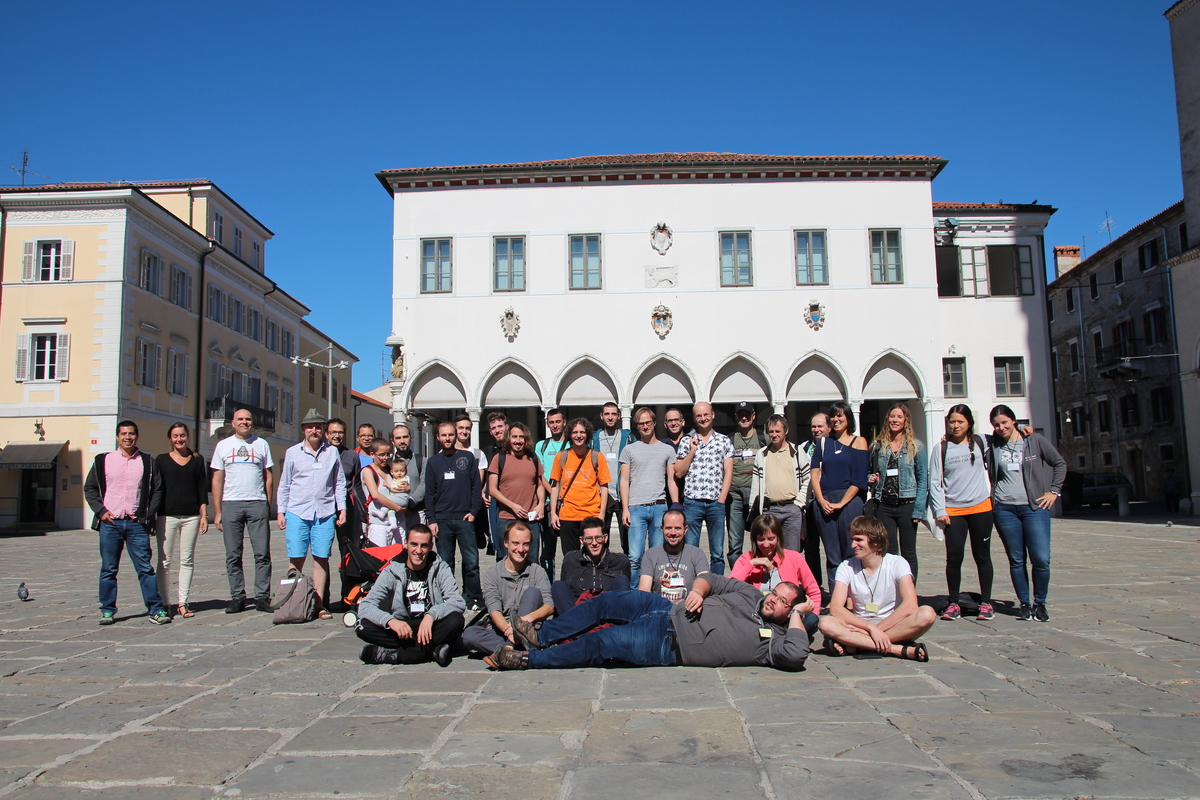
\includegraphics[scale=0.3]{stm-koper2019.jpeg}
\caption*{Software Tools for Mathematics in Koper, Slovenia}
\end{figure}



\end{event}

